\chapter{Les clients}
Les clients sont le cœur de l'application, elle a donc besoin d'ajouter de nouveaux clients pour pouvoir être utilisée. 
\begin{figure}[H]
	\centering
	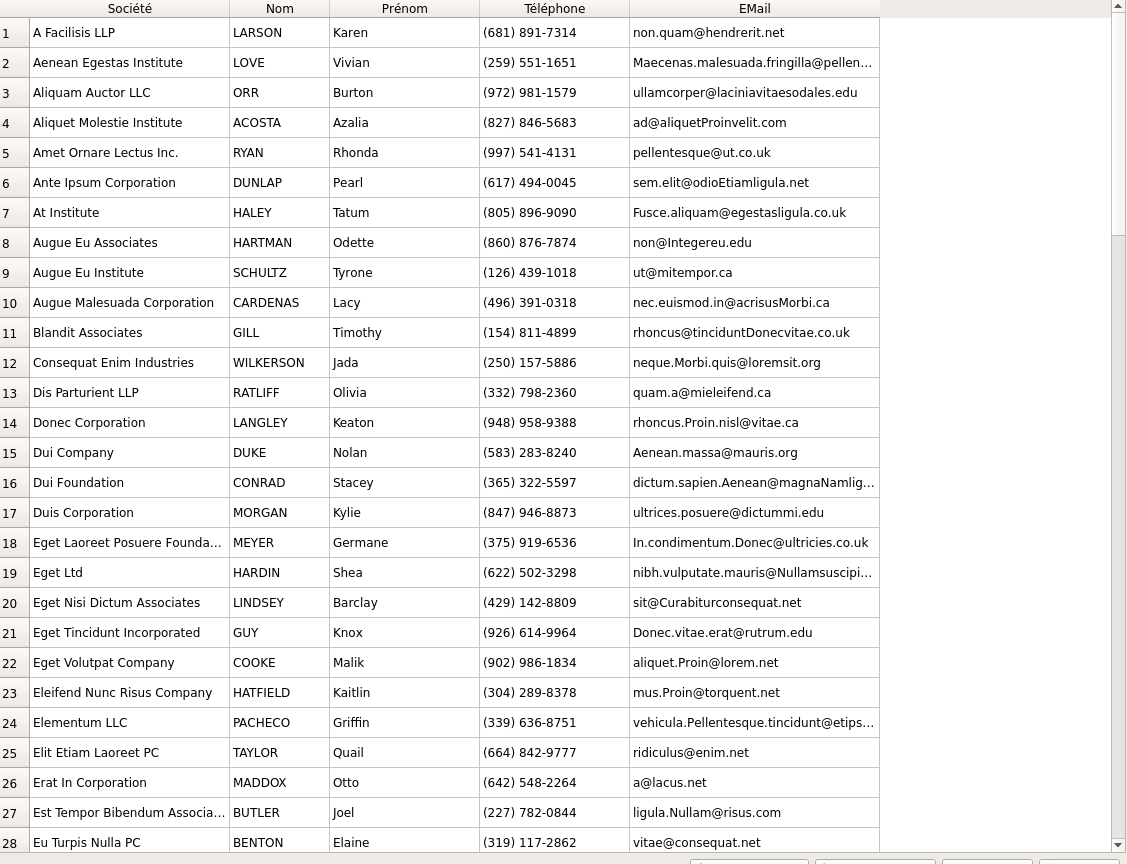
\includegraphics[width=12cm]{screens/clients.png}
	\caption{Gestion des clients}
	\label{fig:gestionClients}
\end{figure}

\section{Liste des clients\index{Client!Liste}}
La liste des clients, cf. figure \ref{fig:gestionClients}, est accessible dès l’ouverture du logiciel. Celle-ci se trouve au centre du logiciel. 

La liste des clients contient uniquement les informations permettant de facilement les identifier à savoir, le nom de la société, le nom,
prénom, le numéro de téléphone et l’adresse e-mail. La sélection dans le tableau de l’un des clients permet, via le panneau du client,
d’obtenir les informations détaillées sur celui-ci. 

\section{Ajout d'un client\index{Client!Ajouter}}
L'ajout d’un client peut se faire via le menu <<Client $\rightarrow$ Nouveau Client>>, via la barre d'outils ou encore via le bouton situé sous la
liste. 
\begin{figure}[H]
	\centering
	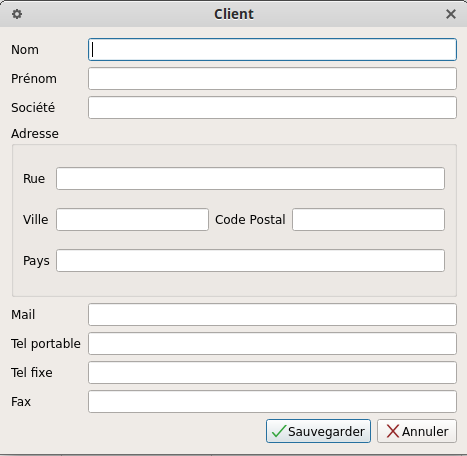
\includegraphics[width=7cm]{screens/ajouterClient.png}
	\caption{Ajouter un client}
\end{figure}

\section{Édition d'un client\index{Client!Éditer}}
L’édition d’un client a pour but de corriger d’éventuelles erreurs sur les informations d’un client. Pour ce faire, il suffit de sélectionner
un client dans le tableau et de cliquer sur le bouton <<Modifier>> situé sous la liste des clients. Il est aussi possible de faire un clic droit sur le client dans le tableau puis, via le menu contextuel, d'"Éditer le client".
 La fenêtre est similaire à celle lors d’un ajout de client, seul diffère les champs qui sont pré-remplis. 

